 



\chapter{The power grid}
%\section{History of the power grid}
%classical power Grid






\section{The Conventional Power Grid}
The \acrfull{cpg} is described in several papers, and books like \cite{BlumeStevenW2007Epsb}, as  a uni-directional, manually controlled, power distribution system.  

\begin{figure}[ht]
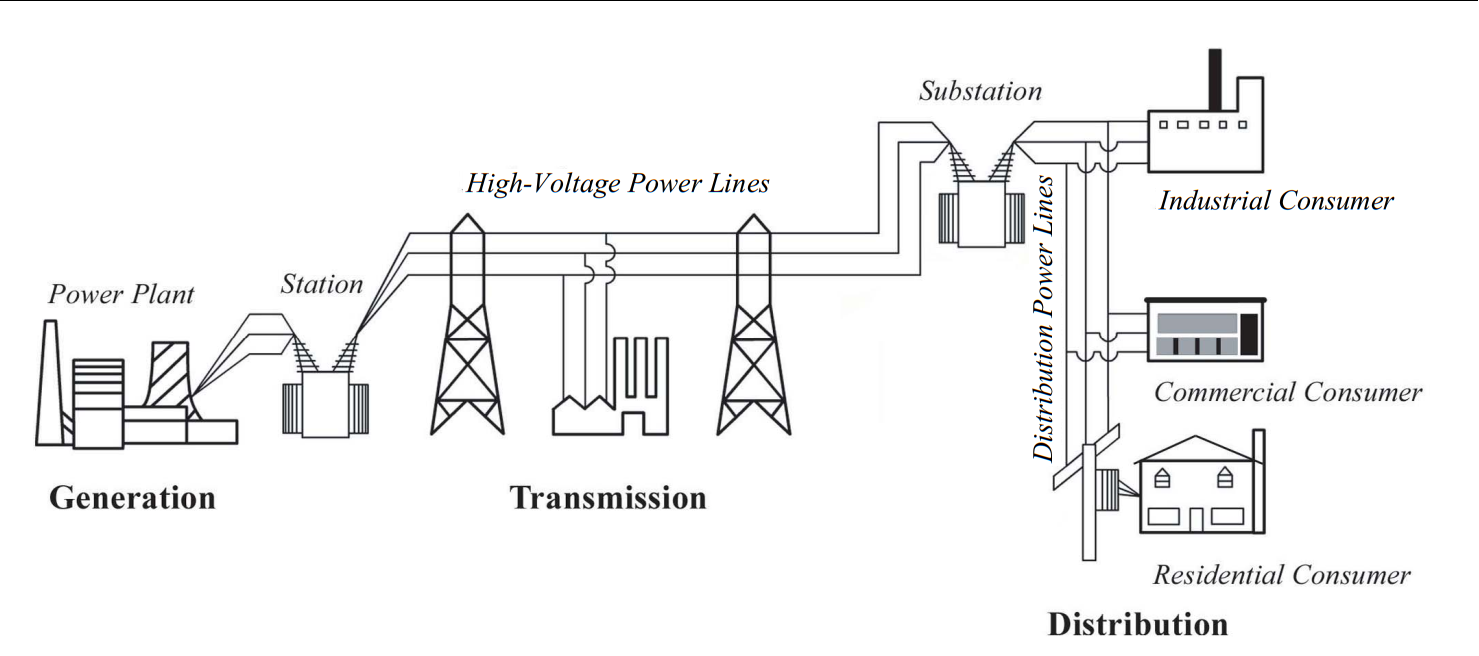
\includegraphics[width=\linewidth]{figures/Blume-PowerGrid-SystemOverView.png}
\caption[Power Grid System Overview]{Power Grid System Overview , as presented in \cite{BlumeStevenW2007Epsb}}
\label{fig:Blume-PowerGrid-SystemOverView}
\end{figure}



\subsection{Overview of the Conventional Power Grid}
The \acrlong{cpg} is a system by which electric power is centrally generated, transmitted, and distributed to industrial, residential,and commercial end users, in order to ensure a reliable access to a sufficient amount of electrical energy. 
\newpage
The \acrlong{cpg}, as described in \cite{BlumeStevenW2007Epsb}, consists of the following subsystems:

\begin{itemize}

 \item The \textbf{Generation Subsystem} which Generates electric power from various sources of energy, to be transmitted for distribution to Consumers. Some examples of installations generating electrical power are nuclear power plants, as well as hydroelectric power plants, feeding water-driven turbines in order to generate power.
 \item The \textbf{Transmission Subsystem} which transmits electric power from the Generation subsystem to the Distribution Subsystem. The current is transmitted via high voltage power lines, minimising energy loss over longer distances.
 \item The \textbf{Distribution Subsystem} which distributes electric power to end users, after converting the high voltage input into lower voltage levels, suitable for consumption.
 \end{itemize}

As described in Chatpter 2.3 of \cite{Rihan2018} %\cite{SmartGridOverview2013}
, the classic \acrshort{pg} is facing challenges, related to Black Outs adhering to the increased demands for electrical power . 


%\section{The Smart Grid}
%smart Grid
\section{The Smart Grid}




In order to provide a description of the \acrfull{sg}, a description of the characteristics of the classic \acrshort{pg} is provided.





As described in  \cite{BlumeStevenW2007Epsb} by \citeauthor{BlumeStevenW2007Epsb}, some of the characteristics of the \acrlong{cpg} are:

\begin{itemize}
\item Power is generated in real time. In the event a consumer is "flipping a power switch," the power grid must have sufficient resources in order to keep the voltage levels at an acceptable level.
\item The Classic \acrlong{pg} is controlled by a central management facility known as the \acrfull{scada} subsystem. The monitoring and management of the \acrshort{pg} is initiated from the Control Center, utilising unidirectional communication channels. 
\item The Classic \acrlong{pg} \acrlong{scada} subsystem is offline, i. e. not connected to any publicly available network. Therefore, operational duties must be performed by personnel physically located at dedicated operational sites.

\end{itemize}

The classic \acrlong{pg} originates from the local society-serving power generation facilities initiating the supply of electrical power, which over the years were interconnected to form a grid, connecting consumers to a network of several power generating facilities, providing a more flexible power distribution infrastructure. 


\subsection{Overview of The Smart Grid}
The \acrshort{sg} is a part of the Critical Infrastructure of a Society, delivering a constant and reliable flow of stable and electrical power to consumers according to demand, in ways both cost efficient and friendly to the environment. The \acrshort{sg} consists of a modernised \acrshort{pg}, under the control of a network based control system. 



As described in \cite{gopstein2021nist}, the following may constitute a definition of the \acrlong{sg}:

\begin{displayquote}[{\cite[p 27]{gopstein2021nist}}]
''A SmartGrid is an electricity network that can intelligently integrate the actions of all
users connected to it - generators, consumers and those that do both – in order to
efficiently deliver sustainable, economic and secure electricity supplies.
A SmartGrid employs innovative products and services together with intelligent monitoring,
control, communication, and self-healing technologies to:
\begin{itemize}
\item better facilitate the connection and operation of generators of all sizes and technologies;
\item allow consumers to play a part in optimizing the operation of the system;
\item provide consumers with greater information and choice of supply;
\item significantly reduce the environmental impact of the whole electricity supply system;
\item deliver enhanced levels of reliability and security of supply.
\end{itemize}
\acrshort{sg} deployment must include not only technology, market and commercial
considerations, environmental impact, regulatory framework, standardization usage, ICT
(Information \& Communication Technology) and migration strategy but also societal
requirements and governmental edicts. 
'' 
\end{displayquote}

The \acrfull{nist} has published a conceptual model of the smart grid, as shown in 
figure \ref{fig:NIST-SmartGRID-ConceptualModel}.



\begin{figure}[ht]
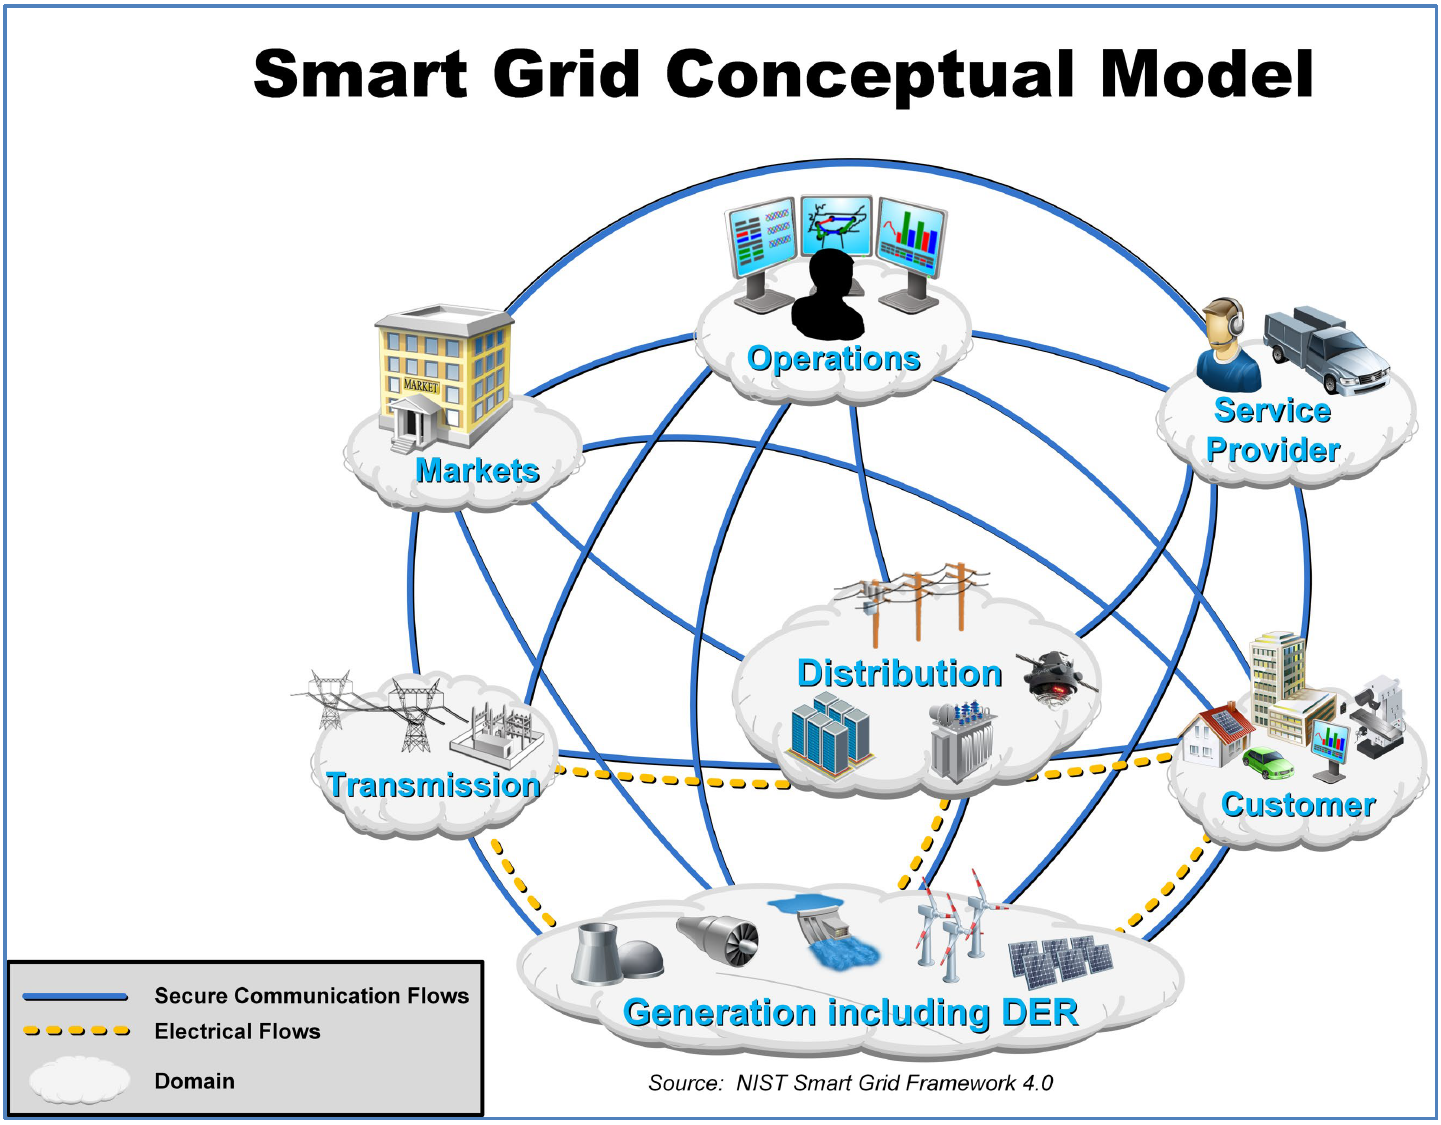
\includegraphics[width=\linewidth]{figures/NIST-SmartGRID-ConceptualModel.png}
\caption[Interactions of roles in SmartGrid Domains]{Interaction of Roles in Different \acrlong{sg} Domains through Secure Communication, as presented in \cite{gopstein2021nist}}
\label{fig:NIST-SmartGRID-ConceptualModel}
\end{figure}






The \acrlong{sg} adds Information and Communication Technology (ICT) to the classic \acrlong{pg}, in order to transform the  unidirectional communication lines of the monitoring and control infrastructure of the \acrlong{cpg}, into an infrastructure utilising two-way communication between the various parts of the \acrlong{sg} infrastructure. 






%\subsection{The Smart Grid: Critical Information Infrastructure}
%According to \cite[p. 610]{Bîrleanu2019}, the \acrlong{sg} consists of the following subsystems:

%\begin{itemize}
%\item \textbf{the classic  power grid}
%\item \textbf{intelligent equipment} 
%\item \textbf{communication infrastructure}
%\end{itemize}

%\cite{Bompard2012}...

%...\acrlong{sg} Subsystems
%\begin{itemize}
%\item 
%\end{itemize}




\subsection{The Smart Grid Domains}




The \acrshort{sg} consists of seven domains, as shown in \figureautorefname { }\ref{fig:NIST-SmartGRID-ConceptualModel}:


    \subsubsection{Customer Domain} The customers are the Consumers of Electricity.
    The power infrastructure of commercial or private customers includes \acrfull{ami}, monitoring the amount of energy consumed, both for billing and \acrfull{dr} purposes. Consumers may plan their consumption, avoiding high-cost periods of heavy load, by  selecting time frames of low prices.
    \subsubsection{Markets Domain} The participants of the Markets Domain aims to balance the consumption and demand of electricity, by adjusting prices on electricity. Price adjustments may be used in order to shift consumption from periods of high demand, to periods of low demand.     
    \subsubsection{Service Provider Domain} Services to the Customers,  as well as the Markets and Operators domain, are provided by the Service Provider Domain, fulfilling duties like customer management and billing, as well as a number of emerging services as required. 
    \subsubsection{Operations Domain} This domain consists of Electricity service operators, ensuring efficient and fail-safe \acrfull{sg} operation, by utilising \acrshort{scada} systems and \acrlong{ems}s in order to monitor and control system operational state.  
    \subsubsection{Bulk Generation Domain} The facilities for producing electricity, resides in this domain. In addition to the connection and interaction with  to the Transmission domain, it interacts with the Markets domain, as well as the operations domain.  
    \subsubsection{Transmission Domain} The actors of the Transmission domain aims to reduce energy loss while transmitting a stable and reliable stream of energy from operators in the bulk generation domain to the distribution domain. The market domain provides input on expected level of demand which may require adjustments of the amount of electricity distributed, controlled and monitored by actors in the operation domain.  
    \subsubsection{Distribution Domain} The actors of the Distribution Domain delivers the electricity to consumers according to demand and availability, and monitors generation and consumption data. Bi-directional power-flow is supported. In the case customers have private  power producing facilities, like solar cells and wind turbines, any surplus electricity might be sold, and distributed to other customers.
